%-------------------------------------------------------------------------------
\section{UCR-131: \ucCXxxiTitle{}(realizaci\'on)}\label{sec:ucr-131}
\textcolor{gray}{V\'ease la especificaci\'on del caso de uso, sec. \ref{uc-131}}\\
\textcolor{gray}{V\'ease el componente main, sec. \ref{sec:cmp-01}}

\paragraph{}
La realizaci\'on del UCR-131 (importaci\'on desde Elasticsearch) es casi la misma que la 
realizaci\'on del UCR-132 (importaci\'on desde OSBs, sec.\ref{sec:ucr-132}):
%
cambia solamente el parser y (obviamente) el main.
El resto del c\'odigo se reutiliza.
El main resuelve las dependencias por medio de inyecci\'on de dependencias,
declaradas en \verb|AppComposer| (no se muestra en el VOPC).

\begin{itemize}
    \item A nivel de BD:
        \begin{itemize}
            \item Alimenta la misma tabla de paso \verb|GMD_NEG_IMPORTA|,
                pero no as\'i la columna \verb|DESC_EXTRAPROYECTOOSB|
                (que es espec\'ifica del OSB, UCR-132)
            \item El stored procedure \verb|PRO_NEG_DEIMPORTAHACIADETALLE|,
                que carga las tablas, 
                carga las mismas tablas excepto \verb|GMD_NEG_SVCOSB|
                (que es espec\'ifica del OSB, UCR-132;
                 detecta los null en \verb|DESC_EXTRAPROYECTOOSB|
                )
        \end{itemize}
    \item A nivel del c\'odigo Java (v\'ease VOPC en fig.\ref{fig:ucr-131-insert}):
        \begin{itemize}
            \item La clase \verb|ESUrlVirtualByDomainJsonParser| parsea 
                el JSON extra\'ido desde Elasticsearch
                (corresponde a \verb|OsbProxyServicesCsvParser|, UCR-132)
            \item Esa clase alimenta la interfaz \verb|CatalogConsumer|
                y \verb|ServiceConsumer| implementadas
                por \verb|BasicServiceInfoImporter|
                (la misma clase ocupada por el OSB Parser, UCR-132)
            \item En realidad \verb|BasicServiceInfoImporter| implementa
                \verb|OsbProxyServiceConsumer| que extiende
                \verb|ServiceConsumer|, pero el c\'odigo discrimina
                la interfaz invocada al no haberse invocado
                \verb|takeOsbProjectName| en el momento de 
                invocar \verb|endService|, lo que finalmente genera la inserci\'on
                de un null en la columna \verb|DESC_EXTRAPROYECTOOSB|
            \item Se ocupa un JsonReader de la librer\'ia Gson,
                para recorrer el JSON en modalidad streaming
                (sin cargarlo entero ya que puede llegar a pesar 3MB),
            \item
                el uso del patr\'on del Consumer permite insertar los datos
                sin pasar por ninguna representaci\'on intermedia
        \end{itemize}
    \item A nivel del JSON:
        \begin{itemize}
            \item El JSON viene enriquecido por el proceso de extracci\'on desde
                Elasticsearch, el cual le agrega la metadata requerida
                por la interfaz \verb|CatalogConsumer|
        \end{itemize}
\end{itemize}


%. . . . . . . . . . . . . . . . . . . . . . . . . . . . . . . . . . . . . . . .
\subsection{UCR-131 VOPC}
\paragraph{}
La figura \ref{fig:ucr-131-insert} muestra las clases que colaboran para cargar
la informaci\'on de Proxy services extra\'ida desde un OSB.
%
La parte de carga de la BD es la misma que el UCR-132 y est\'a descrita en 
la fig.\ref{fig:ucr-132-insert}.

\paragraph{}


\begin{figure}[hbtp]
    \centering
    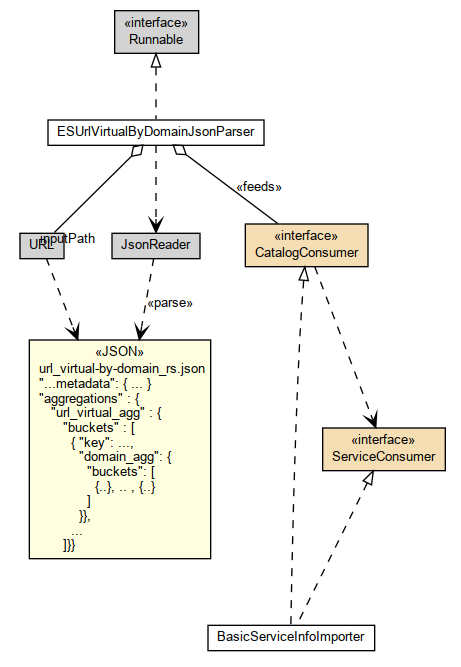
\includegraphics[width=.5\textwidth]{ucr-131-vopc-insert-access_logs-info.png}
    \caption{UC-131 VOPC Carga info URLs y sus dominios desde los logs de acceso, extra\'idos desde Elasticsearch.}
    \label{fig:ucr-131-insert}
\end{figure}
